\chapter{Conceptual Evolution and Rationale}
\label{chap:Conceptual_Evolution_and_Rationale}

This chapter provides a comprehensive analysis of the project's evolution. It delineates the progression from an initial theoretical proposal, through the Self-Sufficiency Raspberry Pi Project, to the final project concept. The discussion elucidates the key motivations, challenges, and pivotal decisions that have ultimately shaped the design.

\section{Introduction}

In the context of this Diploma Thesis, the project has undergone several conceptual transformations aimed at refining its scope, objectives, and implementation strategy. Documenting this evolution is essential for a holistic understanding of the development process, as it highlights the iterative nature of design and the interplay between feasibility, scalability, and the initial research goals. Key considerations included evaluating the project's feasibility, ensuring scalability, and aligning with the overarching research objectives. Additionally, a critical examination of technical challenges encountered during implementation informed subsequent refinements.

\section{Timeline and Milestones}

To provide a clear overview of the project's evolution, a timeline outlining the major milestones, decision points, and revisions is presented in the following chart.
\begin{figure}[H]
    \centering
    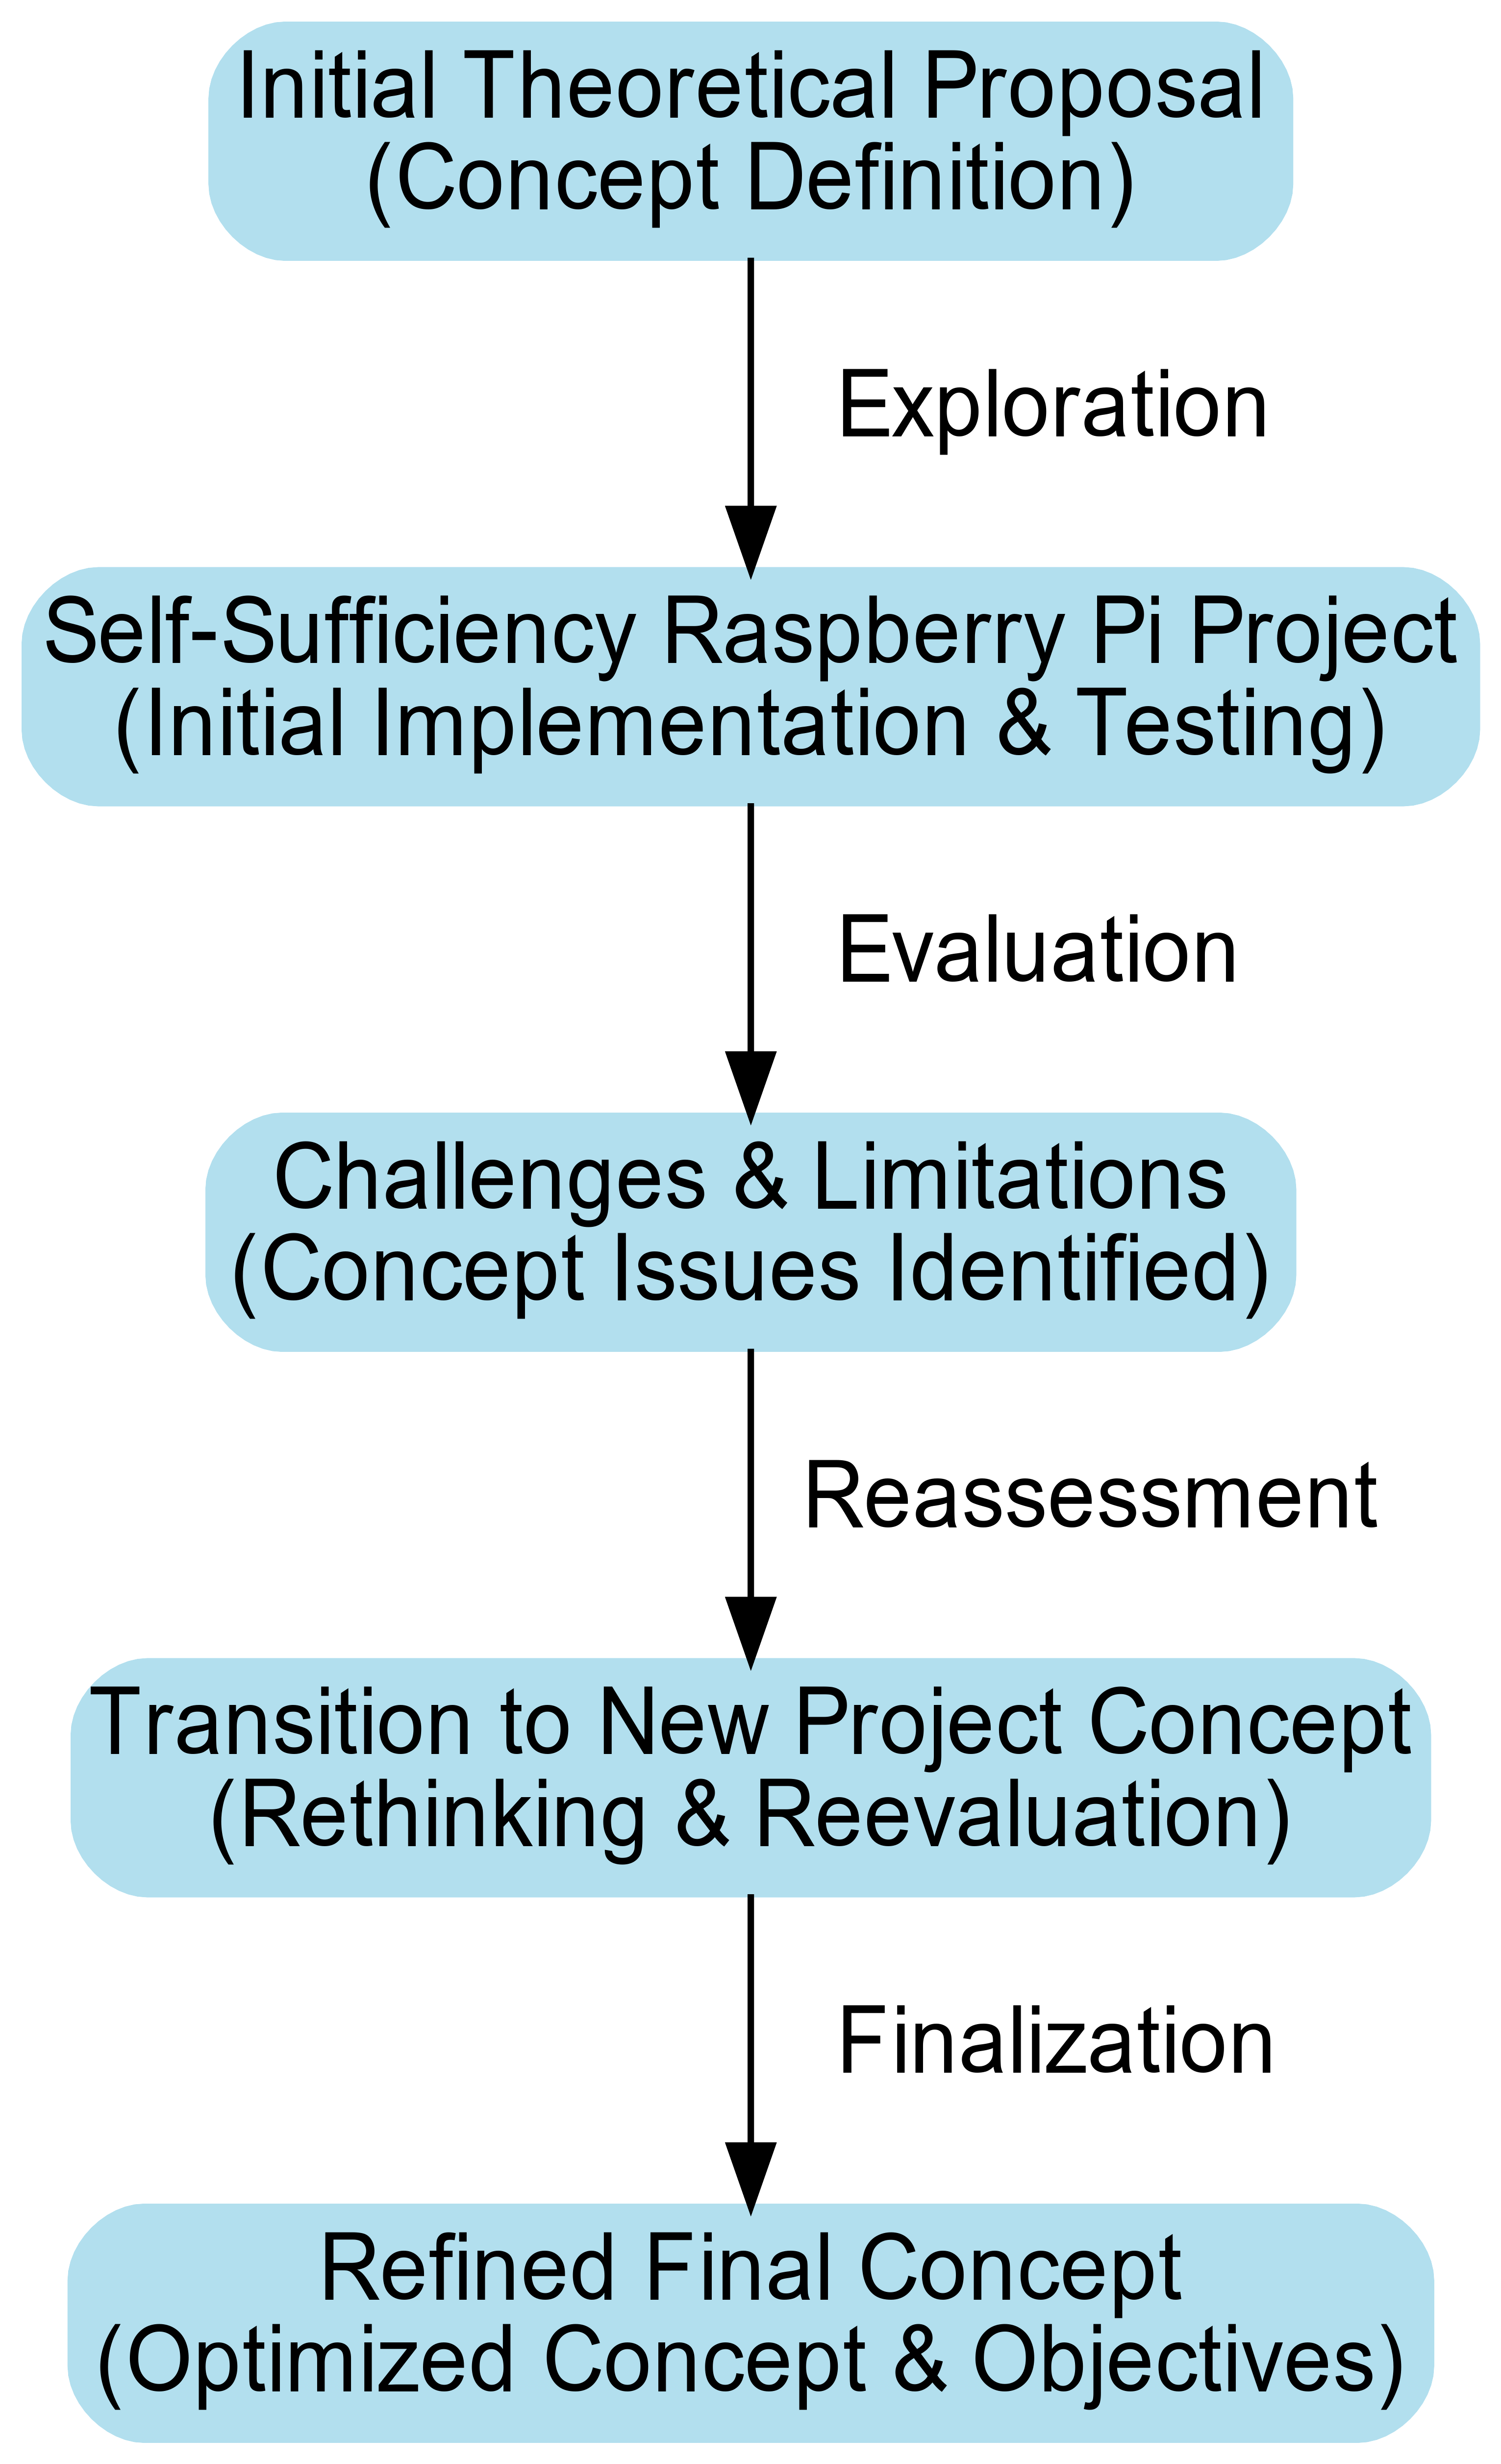
\includegraphics[width=0.4\textwidth]{figures/concept_change_flowchart.png}
    \caption{Gantt Chart of the Project Evolution}
    \label{fig:GanttChart}
\end{figure}

This timeline visually summarizes the progression of ideas and the key changes made over time, offering a concise reference to the project's developmental history.

% ++++++++++++++++++++++++++++++++++++++++++


\section{Initial Concept}

The first concept of the Diploma thesis was to investigate the different methodes how you can leverage AI in different fields 
and also to come up with a way to measure the qualety of the AI model for different tasks and use cases.
The Idea was also to implement questonere to get a better understanding of the different use cases and how the AI model can be used in different fields.
The goal was to come up with a way to measure the qualety of the AI model and to provide a way to compare different models with each other.

But the project team quickly realized that this concept was too broad and that it would be difficult to implement the project in the given time frame.

It is also not very clear how the project should be implemented and how the different parts of the project should be connected to each other.

\section{The Self-Sufficiency Project}

After the initial concept was deemed too broad and complex, the project team decided to focus on a more specific and tangible project idea. 
The Self-Sufficiency Project was born out of the need to create a practical and achievable project that could be implemented within the given time frame.

The idea was to develop a self-sufficient system based on a Raspberry Pi that could perform various tasks that would implement the use of AI models in a practical way.
The self-sufficient part was about trying to eliminate the need of apis and other external services to make the system more robust and independent.

Another key factor of the project idea was to put the whole system in a cariable case so that it could be easily transported and used in different locations.

For a better understanding of the project, the following figure illustrates the conceptual idea of the Self-Sufficiency Rassberry Pi Project.

\begin{figure}[H]
    \centering
    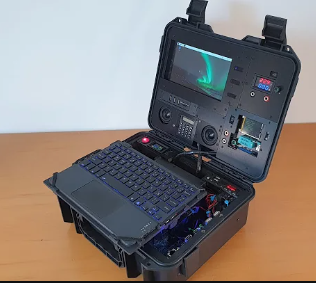
\includegraphics[width=0.5\textwidth]{figures/SAIPIA-concept-picture.png}
    \caption{Conceptual Framework of the Self-Sufficiency Project}
    \label{fig:SelfSufficiencyProject}
\end{figure}


\section{Challenges and Limitations of the Self-Sufficiency Project}

As the project progressed, several challenges and limitations became apparent, prompting a reevaluation of the project's direction. These challenges included:

\begin{itemize}
    \item \textbf{Complexity of Implementation:} The integration of various AI models and hardware components posed significant technical challenges, requiring extensive development and testing.
    \item \textbf{Scalability Concerns:} The self-sufficiency concept limited the project's scalability and interoperability with external systems, potentially hindering future expansion.
    \item \textbf{Resource Constraints:} The project's ambitious scope and resource requirements exceeded the available time and expertise, necessitating a more focused approach.
    \item \textbf{Lack of Clear Objectives:} The project lacked clear, measurable objectives and success criteria, making it challenging to assess progress and outcomes effectively.
    \item \textbf{Integration Complexity:} The integration of AI models, hardware components, and software systems proved more complex than anticipated, requiring a more streamlined approach.
    \item \textbf{Time consernes:} The project team quickly realized that the project would take more time than expected and that it would be difficult to implement the project in the given time frame.
\end{itemize}


Despite its initial promise, the Self-Sufficiency Project encountered several challenges. This section critically examines the practical issues and theoretical shortcomings that led to the reconsideration of the project direction.

\section{Transition to the Current Project Concept}


Based on the analysis of previous limitations, a new project concept was developed. This section explains the rationale behind the transition, details the improvements made, and describes the refined structure of the current project. It also outlines how the different components of the thesis address the project objectives.

\section{Overcoming Challenges in the Current Project Concept}


Every project evolution comes with its own set of challenges. In this section, we identify specific problems encountered in the current project concept and describe the strategies and solutions implemented to resolve them, ensuring the robustness of the final product.

\section{Insights and Lessons Learned}


Reflecting on the entire evolution process, this section summarizes the key insights gained and lessons learned. These reflections serve as guidance for future projects and contribute to a deeper understanding of the iterative design process.

\section{Conclusion}


The chapter concludes by summarizing the journey from the initial concept to the final project idea. It reiterates the importance of adaptive planning and critical analysis in the development process and highlights the contributions of each phase to the overall success of the project.

%###################
